\documentclass[11pt,letterpaper]{report}
\usepackage{amssymb,amsfonts,color,graphicx,amsmath,enumerate}
\usepackage{amsthm}

\newcommand{\naturals}{\mathbb{N}}
\newcommand{\integers}{\mathbb{Z}}
\newcommand{\complex}{\mathbb{C}}
\newcommand{\reals}{\mathbb{R}}
\newcommand{\mcal}[1]{\mathcal{#1}}
\newcommand{\rationals}{\mathbb{Q}}
\newcommand{\field}{\mathbb{F}}
\newcommand{\Var}{\text{Var}}
\newcommand{\ind}{\mathbbm{1}}
\newcommand{\Cov}{\text{Cov}}

\newenvironment{solution}
{\begin{proof}[Solution]}
{\end{proof}}

\voffset=-3cm
\hoffset=-2.25cm
\textheight=24cm
\textwidth=17.25cm
\addtolength{\jot}{8pt}
\linespread{1.3}

\begin{document}
\begin{center}
{\bf \Large 130B - Homework 6}
\vspace{0.2cm}
\hrule
\end{center}

\begin{enumerate}
	\item Suppose we perform a sequence of independent Bernoulli trials, each with success probability $p$. We fix a positive integer $r$ and keep performing trials until we observe $r$ successes. Let $X$ be the random variable that counts the number of trials needed to observe $r$ successes.
	\begin{enumerate}
		\item Compute the probability mass function of $X$,
		\[
		f(k;r,p)= \Pr[X = k].
		\]

		\item Compute the mean and variance of $X$. \textit{Hint: An efficient way to do this is to compute the moments, $E[X^k]$ for any positive integer $k$.}

		\item In words, how is $X$ related to a binomial random variable?
	\end{enumerate}










	\item Suppose we have a bin containing $N$ balls, $m$ of which are red and $N-m$ are blue. Draw a sample of $n$ balls (without replacement) and let $X$ be the number of red balls in the sample.
	\begin{enumerate}
		\item Compute the probability mass function of $X$,
		\[
		f(k; N, m, n) = \Pr[X = k].
		\]

		\item Compute the mean and variance of $X$. \textit{Hint: Same hint as in 1(b).}

		\item In words, how is $X$ related to a binomial random variable?
	\end{enumerate}










	\item Suppose a laser pointer sits at a unit distance from the $x$-axis. We spin the laser about its center and consider the point $X$ at which the beam intersects the $x$-axis once the beam has stopped spinning. If the beam doesn't point toward the $x$-axis, just repeat the experiment.
	\begin{enumerate}
		\item Find the probability density function, $f(x)$, of $X$. The laser setup is illustrated in Figure 1, where $\theta$ is the angle the beam makes with the $y$-axis. Assume that $\theta$ is uniformly distributed between $-\pi/2$ and $\pi/2$.
		\begin{figure}[h]
		\centering
			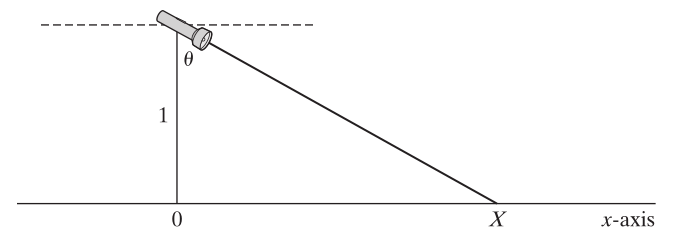
\includegraphics[scale=.6]{beam.PNG}
			\caption{Laser setup}
		\end{figure}

		\item Find the expectation $E[X]$.
	\end{enumerate}










	\item Let $S$ be a semicircle of unit radius on a diameter $D$.
	\begin{enumerate}
		\item A point $P$ is picked at random on $D$. If $X$ is the distance from $P$ to $S$ along the perpendicular to $D$, show that $E[X] = \pi/4$.
		\item A point $Q$ is picked at random on $S$. If $Y$ is the perpendicular distance from $Q$ to $D$, show that $E[Y] = 2/\pi$.
	\end{enumerate}
\end{enumerate}

\end{document}